\section{Results}
\label{sec:results}

\subsection{Scene-text detection}
Some example of the output text instances can be seen in Figure \ref{fig:gen_sample} and \ref{fig:nongen_sample}.

The data was not annotated with bounding boxes of the signage as ground truth for this task, therefore evaluation was done by visual inspection. It was found that the text detection module returned almost all text instances present in the original street view images, including non-horizontal and curved text. Cases where the model failed include very small, and therefore illegible texts; especially in lower resolution images. Additionally, the model also returned some noise, namely texts on street signs (e.g. traffic signs, street names), and watermarks ("©Google", as the images in StreetSwipe were originally from Google Street View) - these instances were manually removed.

\begin{figure}
    \begin{tabular}{cccc}
        \subfloat{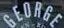
\includegraphics[width = 1.5in]{media/results/instances/gen-8.jpg}} &
        \subfloat{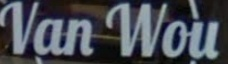
\includegraphics[width = 1.5in]{media/results/instances/gen-2.jpg}} \\
        \subfloat{
\includegraphics[width = 1.5in]{media/results/instances/gen-1.jpg}} &
        \subfloat{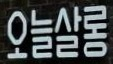
\includegraphics[width = 1.5in]{media/results/instances/gen-4.jpg}} \\
    \end{tabular}
    \caption{Gentrified text instances examples}
    \label{fig:gen_sample}
\end{figure}

\begin{figure}
    \begin{tabular}{cccc}
        \subfloat{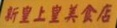
\includegraphics[width = 1.5in]{media/results/instances/non-gen-2.jpg}} &
        \subfloat{
\includegraphics[width = 1.5in]{media/results/instances/non-gen-1.jpg}} \\
        \subfloat{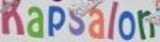
\includegraphics[width = 1.5in]{media/results/instances/non-gen-3.jpg}} &
        \subfloat{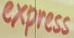
\includegraphics[width = 1.5in]{media/results/instances/non-gen-4.jpg}} \\
    \end{tabular}
    \caption{Non-gentrified text instances examples}
    \label{fig:nongen_sample}
\end{figure}


\subsection{Classification}
\subsubsection{Baseline}
Results of the baseline model are shown in Table \ref{fig:baseline_metrics}.

\begin{table}[h]
\begin{tabular}{llcc}
\multirow{2}{*}{Metrics}   & \multirow{2}{*}{Class} & \multicolumn{2}{c}{Baseline model}        \\ \cline{3-4} 
                           &                        & Classwise & Average                 \\ \hline
Accuracy                   & Gentrified             & 0.2143    & \multirow{2}{*}{0.5810} \\
                           & Non-gentrified         & 0.9478    &                         \\
Precision                  & Gentrified             & 0.6122    & \multirow{2}{*}{0.6852} \\
                           & Non-gentrified         & 0.7582    &                         \\
Recall                     & Gentrified             & 0.2143    & \multirow{2}{*}{0.5810} \\
                           & Non-gentrified         & 0.9478    &                         \\
F1-score                   & Gentrified             & 0.3175    & \multirow{2}{*}{0.5800} \\
                           & Non-gentrified         & 0.8425    &                        
\end{tabular}
\caption{Classwise and macro-averaged metrics of baseline model (ResNet50, no weighted sampling, no fine-tuning). This model achieved very high performance for non-gentrified signage, but performed poorly on gentrified signage, due to class imbalance.}
\label{fig:baseline_metrics}
\end{table}

% \begin{table}[H]
% \begin{tabular}{lcc}
% \multirow{2}{*}{Metrics} & \multicolumn{2}{c}{Baseline} \\ \cline{2-3} 
%                          & Val         & Test           \\ \hline
% Accuracy                 & X           & 0.5810         \\
% Precision                & X           & 0.6852         \\
% Recall                   & X           & 0.5810         \\
% F1-score                 & X           & 0.5800        
% \end{tabular}
% \caption{Macro-averaged metrics of baseline model (ResNet50, no weighted sampling, no fine-tuning)}
% \label{fig:baseline_avg}
% \end{table}

% \begin{table}[H]
% \begin{tabular}{llcc}
% \multirow{2}{*}{Metrics} & \multirow{2}{*}{Class} & \multicolumn{2}{c}{Baseline} \\ \cline{3-4} 
%                          &                        & Val         & Test           \\ \hline
% Accuracy                 & Gentrified             & X           & 0.2143         \\
%                          & Non-gentrified         & X           & 0.9478         \\
% Precision                & Gentrified             & X           & 0.6122         \\
%                          & Non-gentrified         & X           & 0.7582         \\
% Recall                   & Gentrified             & X           & 0.2143         \\
%                          & Non-gentrified         & X           & 0.9478         \\
% F1-score                 & Gentrified             & X           & 0.3175         \\
%                          & Non-gentrified         & X           & 0.8425        
% \end{tabular}
% \caption{Classwise metrics of baseline model (ResNet50, no weighted sampling, no fine-tuning)}
% \label{fig:baseline_cls}
% \end{table}

\subsubsection{Fine-tuned}
The best performing model with ResNet18 architecture was found with learning rate set to 0.001, batch size 32, and 60 training epochs. The best performing model with ResNet50 architecture was found with learning rate set to 0.01, batch size 64, and 60 training epochs. The macro-averaged metrics across classes for these models are shown in Table \ref{fig:resnet_compare}. As can be seen, the fine-tuned ResNet50 has better performance. Its classwise metrics are shown in Table \ref{fig:resnet50_cls}.

\begin{table}[h]
    \begin{tabular}{lcc|cc}
\multirow{2}{*}{Metrics} & \multicolumn{2}{c|}{ResNet18} & \multicolumn{2}{c}{ResNet50} \\ \cline{2-5} 
                         & Val           & Test          & Val           & Test         \\ \hline
Accuracy                 & 0.6497        & 0.6960        & 0.6506        & \textbf{0.7033}       \\
Precision                & 0.6185        & 0.6715        & 0.6209        & \textbf{0.6795}       \\
Recall                   & 0.6497        & 0.6960        & 0.6506        & \textbf{0.7033}       \\
F1-score                 & 0.6222        & 0.6781        & 0.6256        & \textbf{0.6865}      
    \end{tabular}
    \caption{Macro-averaged metrics of the best-performing fine-tuned ResNet18 and ResNet50. Between these two models, the fine-tuned ResNet50 performed better.}
    \label{fig:resnet_compare}
\end{table}


\begin{table}[h]
\begin{tabular}{llcc}
\multirow{2}{*}{Metrics}   & \multirow{2}{*}{Class} & \multicolumn{2}{c}{ResNet50} \\ \cline{3-4} 
                           &                        & Val           & Test         \\ \hline
Accuracy                   & Gentrified             & 0.5714        & 0.6429       \\
                           & Non-gentrified         & 0.7299        & 0.7637       \\
Precision                  & Gentrified             & 0.3953        & 0.5114       \\
                           & Non-gentrified         & 0.8464        & 0.8476       \\
Recall                     & Gentrified             & 0.5714        & 0.6429       \\
                           & Non-gentrified         & 0.7299        & 0.7637       \\
F1-score                   & Gentrified             & 0.4674        & \textbf{0.5696}       \\
                           & Non-gentrified         & 0.7838        & \textbf{0.8035}      
\end{tabular}
\caption{Classwise metrics of best model (fine-tuned ResNet50, learning rate 0.01, batch size 64, 60 epochs). Even though there was clear improvements in classifying gentrified signage compared to the baseline model, this model still did better on non-gentrified signage - most notably shown in the F1-scores of each class.}
\label{fig:resnet50_cls}
\end{table}

\subsection{Testing on extended data}
The average and classwise metrics of the best model in classfying the extended data are presented in Table \ref{fig:resnet50_pano}.

\begin{table}[h]
\begin{tabular}{llcc}
\multirow{2}{*}{Metrics}   & \multirow{2}{*}{Class} & \multicolumn{2}{c}{Extended data}   \\ \cline{3-4} 
                           &                        & Classwise & Average                 \\ \hline
Accuracy                   & Gentrified             & 0.5340    & \multirow{2}{*}{0.5807} \\
                           & Non-gentrified         & 0.6274    &                         \\
Precision                  & Gentrified             & 0.7359    & \multirow{2}{*}{0.5725} \\
                           & Non-gentrified         & 0.4092    &                         \\
Recall                     & Gentrified             & 0.5340    & \multirow{2}{*}{0.5807} \\
                           & Non-gentrified         & 0.6274    &                         \\
F1-score                   & Gentrified             & 0.6189    & \multirow{2}{*}{0.5571} \\
                           & Non-gentrified         & 0.4953    &                        
\end{tabular}
\caption{Average and classwise metrics of the best model in classfying the extended data}
\label{fig:resnet50_pano}
\end{table}

\subsection{Model prediction visualization}
\subsubsection{Correct classifications}
Top 20 samples with the highest probabilities of each class were inspected.

\textit{Gentrified} Correctly classified gentrified signage typically have sans serif fonts. A large portion has white text, background color varies. A larger portion is in English than non-gentrified signs.

\textit{Non-gentrified} Correctly classified non-gentrified signage typically have serif fonts, look more "decorated" with a larger range of colors. Mostly in Dutch.

\subsubsection{Incorrect classifications}
\textit{False gentrified} Signage incorrectly classified as gentrified typically follow the style of correct-gentrified signage: modern and minimalist looking font, also largely white text on dark background or vice versa.

\textit{False non-gentrified} Signage incorrectly classified as non-gentrified also follow the style of correct non-gentrified signage: more decorated fonts, more colors.

\subsubsection{Classifications on extended data}
Also follow the styles of StreetSwipe's gentrified and non-gentrified signage, though more noise and lower resolution.


% \subsection{Clustering signage by visual representation}
% The GMM clustering solution of signage by their vector representations is visualized in Figure \ref{fig:clus_visual}. The silhouette coefficient for this clustering solution is \textit{[...]}, which is \textit{[close to/far from]} 1 and thus signifies a \textit{[clear/unclear]} separation between the two clusters.

% \begin{figure}[b]
%     \centering
%     \includegraphics[width=0.5\textwidth]{media/results/plhldr_clus.png}
%     \caption{[PLACEHOLDER] Signage clustering solution by vector visual representation}
%     \label{fig:clus_visual}
% \end{figure}

% \subsection{Clustering signage by socio-economic indicators}
% The GMM clustering solution of signage by their socio-economic feature vectors is visualized in Figure \ref{fig:clus_indicators}. The silhouette coefficient for this clustering solution is \textit{[...]}, which is \textit{[close to/far from]} 1 and thus signifies a \textit{[clear/unclear]} separation between the two clusters.

% \begin{figure}[b]
%     \centering
%     \includegraphics[width=0.5\textwidth]{media/results/plhldr_clus.png}
%     \caption{[PLACEHOLDER] Signage clustering solution by socio-economic feature vectors}
%     \label{fig:clus_indicators}
% \end{figure}

% \subsection{Clustering solutions agreement}
% The Adjusted Rand Index (ARI) was calculated for the two clustering solution. With a value of \textit{[...]}, the ARI indicates that the clusterings of signage by their visual representation and by their socio-economic indicators \textit{[do/do not]} agree.
